\clearpage
\subsection{Results from "server" [5be79db], generated Wed Oct 19 11:47:49 CEST 2011}
\begin{verbatim}

Test aspects:

    compilation:
        compilation time measured by 'time' call
        only 'real' time is taken into account
        result is in seconds

    size:
        size of the binary measured by 'ls -k' call
        result is in kilobytes

    strip-size:
        size of the binary measured by 'ls -k' call after 'strip' call
        result is in kilobytes

    execution:
        execution time measured by 'time' call
        only 'real' time is taken into account
        result is in seconds

    valgrind:
        test is executed with valgrind call
        result is as A/D (S), where
        A - allocations
        D - deallocations
        S - global allocated size in bytes

    test name:
        test_NAME[_NUMBER], where NAME is test case name and NUMBER is count of event calls during the test
\end{verbatim}
\begin{center}
\line(1,0){750}
\end{center}
\begin{verbatim}

Environment statistics:

    generated: Wed Oct 19 11:47:49 CEST 2011
    code revision: 5be79db
    hostname: "server"
    operating system:  GNU/Linux
    processor: Intel(R) Core(TM)2 Duo CPU P8600 @ 2.40GHz
    free memory: 1229Mb
    load average: 0.79 0.59 0.48 1/307 29073
\end{verbatim}
\begin{center}
\line(1,0){750}
\end{center}
\begin{verbatim}

All tests summary:

    real: 19644.24s (5:27:24)
    user: 19581.76s
    sys: 50.03s
    cpu: 99%
    average memory usage: 0K
    maximum resident set size: 841136K
    number of times the process was swapped out of main memory: 0
    number of file system input: 3008
    number of file system outputs: 309400
\end{verbatim}
\begin{center}
\line(1,0){750}
\end{center}
\begin{verbatim}
Results are presented by using table and types of charts:

    table: contains results for each tested aspect and framework
    first type of chart: presents relative (0-100%) differences between individual framework and aspect
\end{verbatim}
\begin{center}
\line(1,0){750}
\end{center}
\begin{landscape}
\begin{table}
\caption{"server" [5be79db], g++44 -m32 -DNDEBUG -DEXPECTED EVENTS='(2)(109)(137)(157)(179)(197)(227)(241)(269)(283)(313)(347)(367)(389)(419)(977)' -DGIVEN EVENTS='(2)(11)(23)(41)(59)(73)(97)(109)(137)(157)(179)(197)(227)(241)(269)(283)(313)(347)(367)(389)(419)'/test dispatch 10000000}
\centering
\begin{longtable}{| c | c |c |c |c |c |}
\hline
& MetaIfElse& SwitchCase& JumpTable..STD\_MAP& JumpTable..BOOST\_UNORDERED\_MAP& JumpTable..RAW\_TABLE\\
\hline
compilation & 1.08s & 0.90s & 1.16s & 1.34s & 1.09s\\
\hline
size & 80K & 57K & 102K & 117K & 87K\\
\hline
strip-size & 29K & 28K & 36K & 40K & 29K\\
\hline
execution & 3.60s & 2.53s & 5.26s & 5.23s & 2.77s\\
\hline
valgrind & 50/50 (1,624b) & 50/50 (1,624b) & 66/66 (2,032b) & 68/68 (1,964b) & 50/50 (5,624b)\\
\hline
\multicolumn{6}{|c|}{\includegraphics[scale=0.8]{images/"results/server"/"g++44 -m32 -DNDEBUG -DEXPECTED_EVENTS='(2)(109)(137)(157)(179)(197)(227)(241)(269)(283)(313)(347)(367)(389)(419)(977)' -DGIVEN_EVENTS='(2)(11)(23)(41)(59)(73)(97)(109)(137)(157)(179)(197)(227)(241)(269)(283)(313)(347)(367)(389)(419)'"/test_dispatch_10000000_all.png}}\\
\hline
\end{longtable}
\end{table}
\end{landscape}
\begin{landscape}
\begin{table}
\caption{"server" [5be79db], g++44 -m32 -DNDEBUG -DEXPECTED EVENTS='(2)(977)' -DGIVEN EVENTS='(2)(11)(997)'/test dispatch 10000000}
\centering
\begin{longtable}{| c | c |c |c |c |c |}
\hline
& MetaIfElse& SwitchCase& JumpTable..STD\_MAP& JumpTable..BOOST\_UNORDERED\_MAP& JumpTable..RAW\_TABLE\\
\hline
compilation & 1.01s & 0.90s & 1.06s & 1.20s & 1.12s\\
\hline
size & 59K & 52K & 74K & 89K & 60K\\
\hline
strip-size & 26K & 25K & 32K & 36K & 26K\\
\hline
execution & 2.72s & 2.50s & 4.03s & 4.20s & 2.81s\\
\hline
valgrind & 14/14 (1,192b) & 14/14 (1,192b) & 16/16 (1,264b) & 17/17 (1,292b) & 14/14 (5,192b)\\
\hline
\multicolumn{6}{|c|}{\includegraphics[scale=0.8]{images/"results/server"/"g++44 -m32 -DNDEBUG -DEXPECTED_EVENTS='(2)(977)' -DGIVEN_EVENTS='(2)(11)(997)'"/test_dispatch_10000000_all.png}}\\
\hline
\end{longtable}
\end{table}
\end{landscape}
\begin{landscape}
\begin{table}
\caption{"server" [5be79db], g++44 -m32 -DNDEBUG -DEXPECTED EVENTS='(109)(137)(157)(179)(197)(227)(241)(269)(283)(313)(347)' -DGIVEN EVENTS='(109)(137)(157)(179)(197)(227)(241)(269)(283)(313)(347)'/test dispatch 10000000}
\centering
\begin{longtable}{| c | c |c |c |c |c |}
\hline
& MetaIfElse& SwitchCase& JumpTable..STD\_MAP& JumpTable..BOOST\_UNORDERED\_MAP& JumpTable..RAW\_TABLE\\
\hline
compilation & 1.06s & 0.85s & 1.11s & 1.31s & 1.04s\\
\hline
size & 71K & 55K & 90K & 105K & 75K\\
\hline
strip-size & 28K & 26K & 34K & 38K & 28K\\
\hline
execution & 3.13s & 2.51s & 5.55s & 5.26s & 2.84s\\
\hline
valgrind & 30/30 (1,384b) & 30/30 (1,384b) & 41/41 (1,672b) & 43/43 (1,664b) & 30/30 (5,384b)\\
\hline
\multicolumn{6}{|c|}{\includegraphics[scale=0.8]{images/"results/server"/"g++44 -m32 -DNDEBUG -DEXPECTED_EVENTS='(109)(137)(157)(179)(197)(227)(241)(269)(283)(313)(347)' -DGIVEN_EVENTS='(109)(137)(157)(179)(197)(227)(241)(269)(283)(313)(347)'"/test_dispatch_10000000_all.png}}\\
\hline
\end{longtable}
\end{table}
\end{landscape}
\begin{landscape}
\begin{table}
\caption{"server" [5be79db], g++44 -m32 -DNDEBUG -DEXPECTED EVENTS='(109)(137)(157)(179)(197)(227)(241)(269)(283)(313)(347)' -DGIVEN EVENTS='(347)(367)(389)(419)(977)'/test dispatch 10000000}
\centering
\begin{longtable}{| c | c |c |c |c |c |}
\hline
& MetaIfElse& SwitchCase& JumpTable..STD\_MAP& JumpTable..BOOST\_UNORDERED\_MAP& JumpTable..RAW\_TABLE\\
\hline
compilation & 1.06s & 0.89s & 1.10s & 1.35s & 1.05s\\
\hline
size & 71K & 53K & 90K & 105K & 75K\\
\hline
strip-size & 28K & 26K & 34K & 38K & 28K\\
\hline
execution & 3.43s & 2.56s & 4.40s & 4.55s & 2.67s\\
\hline
valgrind & 18/18 (1,240b) & 18/18 (1,240b) & 29/29 (1,528b) & 31/31 (1,520b) & 18/18 (5,240b)\\
\hline
\multicolumn{6}{|c|}{\includegraphics[scale=0.8]{images/"results/server"/"g++44 -m32 -DNDEBUG -DEXPECTED_EVENTS='(109)(137)(157)(179)(197)(227)(241)(269)(283)(313)(347)' -DGIVEN_EVENTS='(347)(367)(389)(419)(977)'"/test_dispatch_10000000_all.png}}\\
\hline
\end{longtable}
\end{table}
\end{landscape}
\begin{landscape}
\begin{table}
\caption{"server" [5be79db], g++44 -m32 -O2 -DNDEBUG -DEXPECTED EVENTS='(2)(109)(137)(157)(179)(197)(227)(241)(269)(283)(313)(347)(367)(389)(419)(977)' -DGIVEN EVENTS='(2)(11)(23)(41)(59)(73)(97)(109)(137)(157)(179)(197)(227)(241)(269)(283)(313)(347)(367)(389)(419)'/test dispatch 10000000}
\centering
\begin{longtable}{| c | c |c |c |c |c |}
\hline
& MetaIfElse& SwitchCase& JumpTable..STD\_MAP& JumpTable..BOOST\_UNORDERED\_MAP& JumpTable..RAW\_TABLE\\
\hline
compilation & 1.25s & 1.08s & 1.40s & 1.61s & 1.27s\\
\hline
size & 22K & 18K & 33K & 32K & 28K\\
\hline
strip-size & 13K & 13K & 18K & 17K & 14K\\
\hline
execution & 0.51s & 0.48s & 0.69s & 0.72s & 0.56s\\
\hline
valgrind & 50/50 (1,624b) & 50/50 (1,624b) & 66/66 (2,032b) & 68/68 (1,964b) & 50/50 (5,624b)\\
\hline
\multicolumn{6}{|c|}{\includegraphics[scale=0.8]{images/"results/server"/"g++44 -m32 -O2 -DNDEBUG -DEXPECTED_EVENTS='(2)(109)(137)(157)(179)(197)(227)(241)(269)(283)(313)(347)(367)(389)(419)(977)' -DGIVEN_EVENTS='(2)(11)(23)(41)(59)(73)(97)(109)(137)(157)(179)(197)(227)(241)(269)(283)(313)(347)(367)(389)(419)'"/test_dispatch_10000000_all.png}}\\
\hline
\end{longtable}
\end{table}
\end{landscape}
\begin{landscape}
\begin{table}
\caption{"server" [5be79db], g++44 -m32 -Os -DNDEBUG -DEXPECTED EVENTS='(2)(109)(137)(157)(179)(197)(227)(241)(269)(283)(313)(347)(367)(389)(419)(977)' -DGIVEN EVENTS='(2)(11)(23)(41)(59)(73)(97)(109)(137)(157)(179)(197)(227)(241)(269)(283)(313)(347)(367)(389)(419)'/test dispatch 10000000}
\centering
\begin{longtable}{| c | c |c |c |c |c |}
\hline
& MetaIfElse& SwitchCase& JumpTable..STD\_MAP& JumpTable..BOOST\_UNORDERED\_MAP& JumpTable..RAW\_TABLE\\
\hline
compilation & 1.01s & 0.88s & 1.21s & 1.40s & 1.09s\\
\hline
size & 19K & 15K & 29K & 29K & 25K\\
\hline
strip-size & 10K & 10K & 12K & 13K & 11K\\
\hline
execution & 0.48s & 0.44s & 0.93s & 0.86s & 0.59s\\
\hline
valgrind & 50/50 (1,624b) & 50/50 (1,624b) & 66/66 (2,032b) & 68/68 (1,964b) & 50/50 (5,624b)\\
\hline
\multicolumn{6}{|c|}{\includegraphics[scale=0.8]{images/"results/server"/"g++44 -m32 -Os -DNDEBUG -DEXPECTED_EVENTS='(2)(109)(137)(157)(179)(197)(227)(241)(269)(283)(313)(347)(367)(389)(419)(977)' -DGIVEN_EVENTS='(2)(11)(23)(41)(59)(73)(97)(109)(137)(157)(179)(197)(227)(241)(269)(283)(313)(347)(367)(389)(419)'"/test_dispatch_10000000_all.png}}\\
\hline
\end{longtable}
\end{table}
\end{landscape}
\begin{landscape}
\begin{table}
\caption{"server" [5be79db], g++44 -m32 -O2 -DNDEBUG -DEXPECTED EVENTS='(2)(977)' -DGIVEN EVENTS='(2)(11)(997)'/test dispatch 10000000}
\centering
\begin{longtable}{| c | c |c |c |c |c |}
\hline
& MetaIfElse& SwitchCase& JumpTable..STD\_MAP& JumpTable..BOOST\_UNORDERED\_MAP& JumpTable..RAW\_TABLE\\
\hline
compilation & 1.09s & 0.99s & 1.41s & 1.37s & 1.03s\\
\hline
size & 17K & 16K & 20K & 21K & 18K\\
\hline
strip-size & 11K & 10K & 13K & 13K & 11K\\
\hline
execution & 0.47s & 0.52s & 0.50s & 0.49s & 0.40s\\
\hline
valgrind & 14/14 (1,192b) & 14/14 (1,192b) & 16/16 (1,264b) & 17/17 (1,292b) & 14/14 (5,192b)\\
\hline
\multicolumn{6}{|c|}{\includegraphics[scale=0.8]{images/"results/server"/"g++44 -m32 -O2 -DNDEBUG -DEXPECTED_EVENTS='(2)(977)' -DGIVEN_EVENTS='(2)(11)(997)'"/test_dispatch_10000000_all.png}}\\
\hline
\end{longtable}
\end{table}
\end{landscape}
\begin{landscape}
\begin{table}
\caption{"server" [5be79db], g++44 -m32 -Os -DNDEBUG -DEXPECTED EVENTS='(2)(977)' -DGIVEN EVENTS='(2)(11)(997)'/test dispatch 10000000}
\centering
\begin{longtable}{| c | c |c |c |c |c |}
\hline
& MetaIfElse& SwitchCase& JumpTable..STD\_MAP& JumpTable..BOOST\_UNORDERED\_MAP& JumpTable..RAW\_TABLE\\
\hline
compilation & 1.00s & 0.89s & 1.02s & 1.27s & 0.96s\\
\hline
size & 16K & 15K & 20K & 21K & 17K\\
\hline
strip-size & 9K & 9K & 11K & 12K & 10K\\
\hline
execution & 0.44s & 0.46s & 0.52s & 0.56s & 0.53s\\
\hline
valgrind & 14/14 (1,192b) & 14/14 (1,192b) & 16/16 (1,264b) & 17/17 (1,292b) & 14/14 (5,192b)\\
\hline
\multicolumn{6}{|c|}{\includegraphics[scale=0.8]{images/"results/server"/"g++44 -m32 -Os -DNDEBUG -DEXPECTED_EVENTS='(2)(977)' -DGIVEN_EVENTS='(2)(11)(997)'"/test_dispatch_10000000_all.png}}\\
\hline
\end{longtable}
\end{table}
\end{landscape}
\begin{landscape}
\begin{table}
\caption{"server" [5be79db], g++44 -m32 -Os -DNDEBUG -DEXPECTED EVENTS='(109)(137)(157)(179)(197)(227)(241)(269)(283)(313)(347)' -DGIVEN EVENTS='(109)(137)(157)(179)(197)(227)(241)(269)(283)(313)(347)'/test dispatch 10000000}
\centering
\begin{longtable}{| c | c |c |c |c |c |}
\hline
& MetaIfElse& SwitchCase& JumpTable..STD\_MAP& JumpTable..BOOST\_UNORDERED\_MAP& JumpTable..RAW\_TABLE\\
\hline
compilation & 0.98s & 0.90s & 1.10s & 1.34s & 1.00s\\
\hline
size & 18K & 15K & 25K & 26K & 22K\\
\hline
strip-size & 10K & 9K & 12K & 12K & 10K\\
\hline
execution & 0.47s & 0.43s & 0.94s & 0.89s & 0.48s\\
\hline
valgrind & 30/30 (1,384b) & 30/30 (1,384b) & 41/41 (1,672b) & 43/43 (1,664b) & 30/30 (5,384b)\\
\hline
\multicolumn{6}{|c|}{\includegraphics[scale=0.8]{images/"results/server"/"g++44 -m32 -Os -DNDEBUG -DEXPECTED_EVENTS='(109)(137)(157)(179)(197)(227)(241)(269)(283)(313)(347)' -DGIVEN_EVENTS='(109)(137)(157)(179)(197)(227)(241)(269)(283)(313)(347)'"/test_dispatch_10000000_all.png}}\\
\hline
\end{longtable}
\end{table}
\end{landscape}
\begin{landscape}
\begin{table}
\caption{"server" [5be79db], g++44 -m32 -O2 -DNDEBUG -DEXPECTED EVENTS='(109)(137)(157)(179)(197)(227)(241)(269)(283)(313)(347)' -DGIVEN EVENTS='(109)(137)(157)(179)(197)(227)(241)(269)(283)(313)(347)'/test dispatch 10000000}
\centering
\begin{longtable}{| c | c |c |c |c |c |}
\hline
& MetaIfElse& SwitchCase& JumpTable..STD\_MAP& JumpTable..BOOST\_UNORDERED\_MAP& JumpTable..RAW\_TABLE\\
\hline
compilation & 1.09s & 1.07s & 1.43s & 1.54s & 1.16s\\
\hline
size & 20K & 17K & 28K & 28K & 23K\\
\hline
strip-size & 12K & 11K & 16K & 15K & 12K\\
\hline
execution & 0.42s & 0.44s & 0.60s & 0.77s & 0.48s\\
\hline
valgrind & 30/30 (1,384b) & 30/30 (1,384b) & 41/41 (1,672b) & 43/43 (1,664b) & 30/30 (5,384b)\\
\hline
\multicolumn{6}{|c|}{\includegraphics[scale=0.8]{images/"results/server"/"g++44 -m32 -O2 -DNDEBUG -DEXPECTED_EVENTS='(109)(137)(157)(179)(197)(227)(241)(269)(283)(313)(347)' -DGIVEN_EVENTS='(109)(137)(157)(179)(197)(227)(241)(269)(283)(313)(347)'"/test_dispatch_10000000_all.png}}\\
\hline
\end{longtable}
\end{table}
\end{landscape}
\begin{landscape}
\begin{table}
\caption{"server" [5be79db], g++44 -m32 -O2 -DNDEBUG -DEXPECTED EVENTS='(109)(137)(157)(179)(197)(227)(241)(269)(283)(313)(347)' -DGIVEN EVENTS='(347)(367)(389)(419)(977)'/test dispatch 10000000}
\centering
\begin{longtable}{| c | c |c |c |c |c |}
\hline
& MetaIfElse& SwitchCase& JumpTable..STD\_MAP& JumpTable..BOOST\_UNORDERED\_MAP& JumpTable..RAW\_TABLE\\
\hline
compilation & 1.06s & 0.98s & 1.18s & 1.45s & 1.13s\\
\hline
size & 19K & 16K & 27K & 27K & 23K\\
\hline
strip-size & 11K & 11K & 15K & 15K & 12K\\
\hline
execution & 0.52s & 0.50s & 0.56s & 0.55s & 0.55s\\
\hline
valgrind & 18/18 (1,240b) & 18/18 (1,240b) & 29/29 (1,528b) & 31/31 (1,520b) & 18/18 (5,240b)\\
\hline
\multicolumn{6}{|c|}{\includegraphics[scale=0.8]{images/"results/server"/"g++44 -m32 -O2 -DNDEBUG -DEXPECTED_EVENTS='(109)(137)(157)(179)(197)(227)(241)(269)(283)(313)(347)' -DGIVEN_EVENTS='(347)(367)(389)(419)(977)'"/test_dispatch_10000000_all.png}}\\
\hline
\end{longtable}
\end{table}
\end{landscape}
\begin{landscape}
\begin{table}
\caption{"server" [5be79db], g++44 -m32 -Os -DNDEBUG -DEXPECTED EVENTS='(109)(137)(157)(179)(197)(227)(241)(269)(283)(313)(347)' -DGIVEN EVENTS='(347)(367)(389)(419)(977)'/test dispatch 10000000}
\centering
\begin{longtable}{| c | c |c |c |c |c |}
\hline
& MetaIfElse& SwitchCase& JumpTable..STD\_MAP& JumpTable..BOOST\_UNORDERED\_MAP& JumpTable..RAW\_TABLE\\
\hline
compilation & 1.09s & 0.85s & 1.08s & 1.35s & 1.10s\\
\hline
size & 18K & 15K & 25K & 26K & 22K\\
\hline
strip-size & 10K & 9K & 12K & 12K & 10K\\
\hline
execution & 0.47s & 0.41s & 0.58s & 0.72s & 0.60s\\
\hline
valgrind & 18/18 (1,240b) & 18/18 (1,240b) & 29/29 (1,528b) & 31/31 (1,520b) & 18/18 (5,240b)\\
\hline
\multicolumn{6}{|c|}{\includegraphics[scale=0.8]{images/"results/server"/"g++44 -m32 -Os -DNDEBUG -DEXPECTED_EVENTS='(109)(137)(157)(179)(197)(227)(241)(269)(283)(313)(347)' -DGIVEN_EVENTS='(347)(367)(389)(419)(977)'"/test_dispatch_10000000_all.png}}\\
\hline
\end{longtable}
\end{table}
\end{landscape}
\begin{landscape}
\begin{table}
\caption{"server" [5be79db], g++34 -m32 -DNDEBUG -DEXPECTED EVENTS='(2)(109)(137)(157)(179)(197)(227)(241)(269)(283)(313)(347)(367)(389)(419)(977)' -DGIVEN EVENTS='(2)(11)(23)(41)(59)(73)(97)(109)(137)(157)(179)(197)(227)(241)(269)(283)(313)(347)(367)(389)(419)'/test dispatch 10000000}
\centering
\begin{longtable}{| c | c |c |c |c |c |}
\hline
& MetaIfElse& SwitchCase& JumpTable..STD\_MAP& JumpTable..BOOST\_UNORDERED\_MAP& JumpTable..RAW\_TABLE\\
\hline
compilation & 1.36s & 1.03s & 1.42s & 1.69s & 1.36s\\
\hline
size & 83K & 60K & 104K & 119K & 90K\\
\hline
strip-size & 32K & 30K & 38K & 43K & 32K\\
\hline
execution & 3.76s & 2.77s & 5.45s & 5.39s & 2.94s\\
\hline
valgrind & 50/50 (1,624b) & 50/50 (1,624b) & 66/66 (2,032b) & 68/68 (1,964b) & 50/50 (5,624b)\\
\hline
\multicolumn{6}{|c|}{\includegraphics[scale=0.8]{images/"results/server"/"g++34 -m32 -DNDEBUG -DEXPECTED_EVENTS='(2)(109)(137)(157)(179)(197)(227)(241)(269)(283)(313)(347)(367)(389)(419)(977)' -DGIVEN_EVENTS='(2)(11)(23)(41)(59)(73)(97)(109)(137)(157)(179)(197)(227)(241)(269)(283)(313)(347)(367)(389)(419)'"/test_dispatch_10000000_all.png}}\\
\hline
\end{longtable}
\end{table}
\end{landscape}
\begin{landscape}
\begin{table}
\caption{"server" [5be79db], g++34 -m32 -DNDEBUG -DEXPECTED EVENTS='(2)(977)' -DGIVEN EVENTS='(2)(11)(997)'/test dispatch 10000000}
\centering
\begin{longtable}{| c | c |c |c |c |c |}
\hline
& MetaIfElse& SwitchCase& JumpTable..STD\_MAP& JumpTable..BOOST\_UNORDERED\_MAP& JumpTable..RAW\_TABLE\\
\hline
compilation & 1.26s & 0.98s & 1.30s & 1.47s & 1.26s\\
\hline
size & 61K & 55K & 75K & 91K & 62K\\
\hline
strip-size & 28K & 27K & 33K & 38K & 28K\\
\hline
execution & 2.96s & 2.75s & 4.19s & 4.34s & 2.89s\\
\hline
valgrind & 14/14 (1,192b) & 14/14 (1,192b) & 16/16 (1,264b) & 17/17 (1,292b) & 14/14 (5,192b)\\
\hline
\multicolumn{6}{|c|}{\includegraphics[scale=0.8]{images/"results/server"/"g++34 -m32 -DNDEBUG -DEXPECTED_EVENTS='(2)(977)' -DGIVEN_EVENTS='(2)(11)(997)'"/test_dispatch_10000000_all.png}}\\
\hline
\end{longtable}
\end{table}
\end{landscape}
\begin{landscape}
\begin{table}
\caption{"server" [5be79db], g++34 -m32 -DNDEBUG -DEXPECTED EVENTS='(109)(137)(157)(179)(197)(227)(241)(269)(283)(313)(347)' -DGIVEN EVENTS='(109)(137)(157)(179)(197)(227)(241)(269)(283)(313)(347)'/test dispatch 10000000}
\centering
\begin{longtable}{| c | c |c |c |c |c |}
\hline
& MetaIfElse& SwitchCase& JumpTable..STD\_MAP& JumpTable..BOOST\_UNORDERED\_MAP& JumpTable..RAW\_TABLE\\
\hline
compilation & 1.33s & 1.00s & 1.30s & 1.59s & 1.33s\\
\hline
size & 74K & 57K & 92K & 107K & 78K\\
\hline
strip-size & 30K & 29K & 36K & 41K & 30K\\
\hline
execution & 3.32s & 2.71s & 5.77s & 5.48s & 3.05s\\
\hline
valgrind & 30/30 (1,384b) & 30/30 (1,384b) & 41/41 (1,672b) & 43/43 (1,664b) & 30/30 (5,384b)\\
\hline
\multicolumn{6}{|c|}{\includegraphics[scale=0.8]{images/"results/server"/"g++34 -m32 -DNDEBUG -DEXPECTED_EVENTS='(109)(137)(157)(179)(197)(227)(241)(269)(283)(313)(347)' -DGIVEN_EVENTS='(109)(137)(157)(179)(197)(227)(241)(269)(283)(313)(347)'"/test_dispatch_10000000_all.png}}\\
\hline
\end{longtable}
\end{table}
\end{landscape}
\begin{landscape}
\begin{table}
\caption{"server" [5be79db], g++34 -m32 -DNDEBUG -DEXPECTED EVENTS='(109)(137)(157)(179)(197)(227)(241)(269)(283)(313)(347)' -DGIVEN EVENTS='(347)(367)(389)(419)(977)'/test dispatch 10000000}
\centering
\begin{longtable}{| c | c |c |c |c |c |}
\hline
& MetaIfElse& SwitchCase& JumpTable..STD\_MAP& JumpTable..BOOST\_UNORDERED\_MAP& JumpTable..RAW\_TABLE\\
\hline
compilation & 1.31s & 0.96s & 1.42s & 1.61s & 1.34s\\
\hline
size & 74K & 55K & 91K & 107K & 78K\\
\hline
strip-size & 30K & 28K & 36K & 41K & 30K\\
\hline
execution & 3.70s & 2.72s & 4.32s & 4.47s & 2.86s\\
\hline
valgrind & 18/18 (1,240b) & 18/18 (1,240b) & 29/29 (1,528b) & 31/31 (1,520b) & 18/18 (5,240b)\\
\hline
\multicolumn{6}{|c|}{\includegraphics[scale=0.8]{images/"results/server"/"g++34 -m32 -DNDEBUG -DEXPECTED_EVENTS='(109)(137)(157)(179)(197)(227)(241)(269)(283)(313)(347)' -DGIVEN_EVENTS='(347)(367)(389)(419)(977)'"/test_dispatch_10000000_all.png}}\\
\hline
\end{longtable}
\end{table}
\end{landscape}
\begin{landscape}
\begin{table}
\caption{"server" [5be79db], g++34 -m32 -O2 -DNDEBUG -DEXPECTED EVENTS='(2)(109)(137)(157)(179)(197)(227)(241)(269)(283)(313)(347)(367)(389)(419)(977)' -DGIVEN EVENTS='(2)(11)(23)(41)(59)(73)(97)(109)(137)(157)(179)(197)(227)(241)(269)(283)(313)(347)(367)(389)(419)'/test dispatch 10000000}
\centering
\begin{longtable}{| c | c |c |c |c |c |}
\hline
& MetaIfElse& SwitchCase& JumpTable..STD\_MAP& JumpTable..BOOST\_UNORDERED\_MAP& JumpTable..RAW\_TABLE\\
\hline
compilation & 1.53s & 1.16s & 1.64s & 1.85s & 1.51s\\
\hline
size & 23K & 19K & 33K & 34K & 29K\\
\hline
strip-size & 14K & 13K & 18K & 19K & 14K\\
\hline
execution & 0.53s & 0.47s & 0.89s & 0.82s & 0.57s\\
\hline
valgrind & 50/50 (1,624b) & 50/50 (1,624b) & 66/66 (2,032b) & 68/68 (1,964b) & 50/50 (5,624b)\\
\hline
\multicolumn{6}{|c|}{\includegraphics[scale=0.8]{images/"results/server"/"g++34 -m32 -O2 -DNDEBUG -DEXPECTED_EVENTS='(2)(109)(137)(157)(179)(197)(227)(241)(269)(283)(313)(347)(367)(389)(419)(977)' -DGIVEN_EVENTS='(2)(11)(23)(41)(59)(73)(97)(109)(137)(157)(179)(197)(227)(241)(269)(283)(313)(347)(367)(389)(419)'"/test_dispatch_10000000_all.png}}\\
\hline
\end{longtable}
\end{table}
\end{landscape}
\begin{landscape}
\begin{table}
\caption{"server" [5be79db], g++34 -m32 -Os -DNDEBUG -DEXPECTED EVENTS='(2)(109)(137)(157)(179)(197)(227)(241)(269)(283)(313)(347)(367)(389)(419)(977)' -DGIVEN EVENTS='(2)(11)(23)(41)(59)(73)(97)(109)(137)(157)(179)(197)(227)(241)(269)(283)(313)(347)(367)(389)(419)'/test dispatch 10000000}
\centering
\begin{longtable}{| c | c |c |c |c |c |}
\hline
& MetaIfElse& SwitchCase& JumpTable..STD\_MAP& JumpTable..BOOST\_UNORDERED\_MAP& JumpTable..RAW\_TABLE\\
\hline
compilation & 1.51s & 1.14s & 1.63s & 1.85s & 1.50s\\
\hline
size & 22K & 18K & 32K & 32K & 28K\\
\hline
strip-size & 13K & 12K & 17K & 17K & 13K\\
\hline
execution & 0.55s & 0.49s & 1.02s & 0.90s & 0.51s\\
\hline
valgrind & 50/50 (1,624b) & 50/50 (1,624b) & 66/66 (2,032b) & 68/68 (1,964b) & 50/50 (5,624b)\\
\hline
\multicolumn{6}{|c|}{\includegraphics[scale=0.8]{images/"results/server"/"g++34 -m32 -Os -DNDEBUG -DEXPECTED_EVENTS='(2)(109)(137)(157)(179)(197)(227)(241)(269)(283)(313)(347)(367)(389)(419)(977)' -DGIVEN_EVENTS='(2)(11)(23)(41)(59)(73)(97)(109)(137)(157)(179)(197)(227)(241)(269)(283)(313)(347)(367)(389)(419)'"/test_dispatch_10000000_all.png}}\\
\hline
\end{longtable}
\end{table}
\end{landscape}
\begin{landscape}
\begin{table}
\caption{"server" [5be79db], g++34 -m32 -O2 -DNDEBUG -DEXPECTED EVENTS='(2)(977)' -DGIVEN EVENTS='(2)(11)(997)'/test dispatch 10000000}
\centering
\begin{longtable}{| c | c |c |c |c |c |}
\hline
& MetaIfElse& SwitchCase& JumpTable..STD\_MAP& JumpTable..BOOST\_UNORDERED\_MAP& JumpTable..RAW\_TABLE\\
\hline
compilation & 1.35s & 1.09s & 1.46s & 1.65s & 1.36s\\
\hline
size & 19K & 18K & 23K & 25K & 20K\\
\hline
strip-size & 13K & 12K & 15K & 16K & 13K\\
\hline
execution & 0.49s & 0.50s & 0.61s & 0.67s & 0.58s\\
\hline
valgrind & 14/14 (1,192b) & 14/14 (1,192b) & 16/16 (1,264b) & 17/17 (1,292b) & 14/14 (5,192b)\\
\hline
\multicolumn{6}{|c|}{\includegraphics[scale=0.8]{images/"results/server"/"g++34 -m32 -O2 -DNDEBUG -DEXPECTED_EVENTS='(2)(977)' -DGIVEN_EVENTS='(2)(11)(997)'"/test_dispatch_10000000_all.png}}\\
\hline
\end{longtable}
\end{table}
\end{landscape}
\begin{landscape}
\begin{table}
\caption{"server" [5be79db], g++34 -m32 -Os -DNDEBUG -DEXPECTED EVENTS='(2)(977)' -DGIVEN EVENTS='(2)(11)(997)'/test dispatch 10000000}
\centering
\begin{longtable}{| c | c |c |c |c |c |}
\hline
& MetaIfElse& SwitchCase& JumpTable..STD\_MAP& JumpTable..BOOST\_UNORDERED\_MAP& JumpTable..RAW\_TABLE\\
\hline
compilation & 1.39s & 1.09s & 1.45s & 1.73s & 1.36s\\
\hline
size & 18K & 17K & 22K & 23K & 19K\\
\hline
strip-size & 12K & 12K & 14K & 15K & 12K\\
\hline
execution & 0.49s & 0.52s & 0.69s & 0.64s & 0.55s\\
\hline
valgrind & 14/14 (1,192b) & 14/14 (1,192b) & 16/16 (1,264b) & 17/17 (1,292b) & 14/14 (5,192b)\\
\hline
\multicolumn{6}{|c|}{\includegraphics[scale=0.8]{images/"results/server"/"g++34 -m32 -Os -DNDEBUG -DEXPECTED_EVENTS='(2)(977)' -DGIVEN_EVENTS='(2)(11)(997)'"/test_dispatch_10000000_all.png}}\\
\hline
\end{longtable}
\end{table}
\end{landscape}
\begin{landscape}
\begin{table}
\caption{"server" [5be79db], g++34 -m32 -O2 -DNDEBUG -DEXPECTED EVENTS='(109)(137)(157)(179)(197)(227)(241)(269)(283)(313)(347)' -DGIVEN EVENTS='(109)(137)(157)(179)(197)(227)(241)(269)(283)(313)(347)'/test dispatch 10000000}
\centering
\begin{longtable}{| c | c |c |c |c |c |}
\hline
& MetaIfElse& SwitchCase& JumpTable..STD\_MAP& JumpTable..BOOST\_UNORDERED\_MAP& JumpTable..RAW\_TABLE\\
\hline
compilation & 1.46s & 1.24s & 1.59s & 1.73s & 1.48s\\
\hline
size & 21K & 18K & 29K & 30K & 25K\\
\hline
strip-size & 14K & 13K & 17K & 18K & 14K\\
\hline
execution & 0.42s & 0.46s & 0.96s & 0.87s & 0.54s\\
\hline
valgrind & 30/30 (1,384b) & 30/30 (1,384b) & 41/41 (1,672b) & 43/43 (1,664b) & 30/30 (5,384b)\\
\hline
\multicolumn{6}{|c|}{\includegraphics[scale=0.8]{images/"results/server"/"g++34 -m32 -O2 -DNDEBUG -DEXPECTED_EVENTS='(109)(137)(157)(179)(197)(227)(241)(269)(283)(313)(347)' -DGIVEN_EVENTS='(109)(137)(157)(179)(197)(227)(241)(269)(283)(313)(347)'"/test_dispatch_10000000_all.png}}\\
\hline
\end{longtable}
\end{table}
\end{landscape}
\begin{landscape}
\begin{table}
\caption{"server" [5be79db], g++34 -m32 -Os -DNDEBUG -DEXPECTED EVENTS='(109)(137)(157)(179)(197)(227)(241)(269)(283)(313)(347)' -DGIVEN EVENTS='(109)(137)(157)(179)(197)(227)(241)(269)(283)(313)(347)'/test dispatch 10000000}
\centering
\begin{longtable}{| c | c |c |c |c |c |}
\hline
& MetaIfElse& SwitchCase& JumpTable..STD\_MAP& JumpTable..BOOST\_UNORDERED\_MAP& JumpTable..RAW\_TABLE\\
\hline
compilation & 1.44s & 1.06s & 1.56s & 1.81s & 1.40s\\
\hline
size & 21K & 17K & 28K & 29K & 24K\\
\hline
strip-size & 13K & 12K & 16K & 16K & 13K\\
\hline
execution & 0.54s & 0.46s & 1.13s & 0.97s & 0.44s\\
\hline
valgrind & 30/30 (1,384b) & 30/30 (1,384b) & 41/41 (1,672b) & 43/43 (1,664b) & 30/30 (5,384b)\\
\hline
\multicolumn{6}{|c|}{\includegraphics[scale=0.8]{images/"results/server"/"g++34 -m32 -Os -DNDEBUG -DEXPECTED_EVENTS='(109)(137)(157)(179)(197)(227)(241)(269)(283)(313)(347)' -DGIVEN_EVENTS='(109)(137)(157)(179)(197)(227)(241)(269)(283)(313)(347)'"/test_dispatch_10000000_all.png}}\\
\hline
\end{longtable}
\end{table}
\end{landscape}
\begin{landscape}
\begin{table}
\caption{"server" [5be79db], g++34 -m32 -O2 -DNDEBUG -DEXPECTED EVENTS='(109)(137)(157)(179)(197)(227)(241)(269)(283)(313)(347)' -DGIVEN EVENTS='(347)(367)(389)(419)(977)'/test dispatch 10000000}
\centering
\begin{longtable}{| c | c |c |c |c |c |}
\hline
& MetaIfElse& SwitchCase& JumpTable..STD\_MAP& JumpTable..BOOST\_UNORDERED\_MAP& JumpTable..RAW\_TABLE\\
\hline
compilation & 1.47s & 1.10s & 1.49s & 1.82s & 1.38s\\
\hline
size & 21K & 18K & 28K & 29K & 24K\\
\hline
strip-size & 13K & 12K & 16K & 17K & 13K\\
\hline
execution & 0.52s & 0.47s & 0.65s & 0.67s & 0.56s\\
\hline
valgrind & 18/18 (1,240b) & 18/18 (1,240b) & 29/29 (1,528b) & 31/31 (1,520b) & 18/18 (5,240b)\\
\hline
\multicolumn{6}{|c|}{\includegraphics[scale=0.8]{images/"results/server"/"g++34 -m32 -O2 -DNDEBUG -DEXPECTED_EVENTS='(109)(137)(157)(179)(197)(227)(241)(269)(283)(313)(347)' -DGIVEN_EVENTS='(347)(367)(389)(419)(977)'"/test_dispatch_10000000_all.png}}\\
\hline
\end{longtable}
\end{table}
\end{landscape}
\begin{landscape}
\begin{table}
\caption{"server" [5be79db], g++34 -m32 -Os -DNDEBUG -DEXPECTED EVENTS='(109)(137)(157)(179)(197)(227)(241)(269)(283)(313)(347)' -DGIVEN EVENTS='(347)(367)(389)(419)(977)'/test dispatch 10000000}
\centering
\begin{longtable}{| c | c |c |c |c |c |}
\hline
& MetaIfElse& SwitchCase& JumpTable..STD\_MAP& JumpTable..BOOST\_UNORDERED\_MAP& JumpTable..RAW\_TABLE\\
\hline
compilation & 1.43s & 1.04s & 1.53s & 1.77s & 1.44s\\
\hline
size & 20K & 17K & 27K & 28K & 24K\\
\hline
strip-size & 12K & 12K & 15K & 16K & 13K\\
\hline
execution & 0.50s & 0.51s & 0.68s & 0.74s & 0.52s\\
\hline
valgrind & 18/18 (1,240b) & 18/18 (1,240b) & 29/29 (1,528b) & 31/31 (1,520b) & 18/18 (5,240b)\\
\hline
\multicolumn{6}{|c|}{\includegraphics[scale=0.8]{images/"results/server"/"g++34 -m32 -Os -DNDEBUG -DEXPECTED_EVENTS='(109)(137)(157)(179)(197)(227)(241)(269)(283)(313)(347)' -DGIVEN_EVENTS='(347)(367)(389)(419)(977)'"/test_dispatch_10000000_all.png}}\\
\hline
\end{longtable}
\end{table}
\end{landscape}
\begin{landscape}
\begin{table}
\caption{"server" [5be79db], g++44 -m32 -g -DEXPECTED EVENTS='(2)(109)(137)(157)(179)(197)(227)(241)(269)(283)(313)(347)(367)(389)(419)(977)' -DGIVEN EVENTS='(2)(11)(23)(41)(59)(73)(97)(109)(137)(157)(179)(197)(227)(241)(269)(283)(313)(347)(367)(389)(419)'/test dispatch 10000000}
\centering
\begin{longtable}{| c | c |c |c |c |c |}
\hline
& MetaIfElse& SwitchCase& JumpTable..STD\_MAP& JumpTable..BOOST\_UNORDERED\_MAP& JumpTable..RAW\_TABLE\\
\hline
compilation & 1.24s & 1.01s & 1.35s & 1.54s & 1.22s\\
\hline
size & 365K & 249K & 460K & 541K & 390K\\
\hline
strip-size & 30K & 28K & 37K & 43K & 30K\\
\hline
execution & 3.51s & 2.70s & 5.28s & 5.14s & 2.80s\\
\hline
valgrind & 50/50 (1,624b) & 50/50 (1,624b) & 66/66 (2,032b) & 68/68 (1,964b) & 50/50 (5,624b)\\
\hline
\multicolumn{6}{|c|}{\includegraphics[scale=0.8]{images/"results/server"/"g++44 -m32 -g -DEXPECTED_EVENTS='(2)(109)(137)(157)(179)(197)(227)(241)(269)(283)(313)(347)(367)(389)(419)(977)' -DGIVEN_EVENTS='(2)(11)(23)(41)(59)(73)(97)(109)(137)(157)(179)(197)(227)(241)(269)(283)(313)(347)(367)(389)(419)'"/test_dispatch_10000000_all.png}}\\
\hline
\end{longtable}
\end{table}
\end{landscape}
\begin{landscape}
\begin{table}
\caption{"server" [5be79db], g++44 -m32 -g -DEXPECTED EVENTS='(2)(977)' -DGIVEN EVENTS='(2)(11)(997)'/test dispatch 10000000}
\centering
\begin{longtable}{| c | c |c |c |c |c |}
\hline
& MetaIfElse& SwitchCase& JumpTable..STD\_MAP& JumpTable..BOOST\_UNORDERED\_MAP& JumpTable..RAW\_TABLE\\
\hline
compilation & 1.11s & 0.94s & 1.20s & 2.41s & 1.22s\\
\hline
size & 264K & 232K & 338K & 419K & 269K\\
\hline
strip-size & 26K & 26K & 33K & 39K & 27K\\
\hline
execution & 2.78s & 2.60s & 3.97s & 4.28s & 2.73s\\
\hline
valgrind & 14/14 (1,192b) & 14/14 (1,192b) & 16/16 (1,264b) & 17/17 (1,292b) & 14/14 (5,192b)\\
\hline
\multicolumn{6}{|c|}{\includegraphics[scale=0.8]{images/"results/server"/"g++44 -m32 -g -DEXPECTED_EVENTS='(2)(977)' -DGIVEN_EVENTS='(2)(11)(997)'"/test_dispatch_10000000_all.png}}\\
\hline
\end{longtable}
\end{table}
\end{landscape}
\begin{landscape}
\begin{table}
\caption{"server" [5be79db], g++44 -m32 -g -DEXPECTED EVENTS='(109)(137)(157)(179)(197)(227)(241)(269)(283)(313)(347)' -DGIVEN EVENTS='(109)(137)(157)(179)(197)(227)(241)(269)(283)(313)(347)'/test dispatch 10000000}
\centering
\begin{longtable}{| c | c |c |c |c |c |}
\hline
& MetaIfElse& SwitchCase& JumpTable..STD\_MAP& JumpTable..BOOST\_UNORDERED\_MAP& JumpTable..RAW\_TABLE\\
\hline
compilation & 1.11s & 1.03s & 1.17s & 1.53s & 1.22s\\
\hline
size & 321K & 239K & 407K & 488K & 337K\\
\hline
strip-size & 29K & 27K & 35K & 41K & 29K\\
\hline
execution & 3.06s & 2.61s & 5.54s & 5.38s & 2.83s\\
\hline
valgrind & 30/30 (1,384b) & 30/30 (1,384b) & 41/41 (1,672b) & 43/43 (1,664b) & 30/30 (5,384b)\\
\hline
\multicolumn{6}{|c|}{\includegraphics[scale=0.8]{images/"results/server"/"g++44 -m32 -g -DEXPECTED_EVENTS='(109)(137)(157)(179)(197)(227)(241)(269)(283)(313)(347)' -DGIVEN_EVENTS='(109)(137)(157)(179)(197)(227)(241)(269)(283)(313)(347)'"/test_dispatch_10000000_all.png}}\\
\hline
\end{longtable}
\end{table}
\end{landscape}
\begin{landscape}
\begin{table}
\caption{"server" [5be79db], g++44 -m32 -g -DEXPECTED EVENTS='(109)(137)(157)(179)(197)(227)(241)(269)(283)(313)(347)' -DGIVEN EVENTS='(347)(367)(389)(419)(977)'/test dispatch 10000000}
\centering
\begin{longtable}{| c | c |c |c |c |c |}
\hline
& MetaIfElse& SwitchCase& JumpTable..STD\_MAP& JumpTable..BOOST\_UNORDERED\_MAP& JumpTable..RAW\_TABLE\\
\hline
compilation & 1.19s & 0.99s & 1.40s & 1.50s & 1.22s\\
\hline
size & 321K & 233K & 407K & 488K & 337K\\
\hline
strip-size & 29K & 26K & 35K & 41K & 29K\\
\hline
execution & 3.41s & 2.61s & 4.44s & 4.38s & 2.69s\\
\hline
valgrind & 18/18 (1,240b) & 18/18 (1,240b) & 29/29 (1,528b) & 31/31 (1,520b) & 18/18 (5,240b)\\
\hline
\multicolumn{6}{|c|}{\includegraphics[scale=0.8]{images/"results/server"/"g++44 -m32 -g -DEXPECTED_EVENTS='(109)(137)(157)(179)(197)(227)(241)(269)(283)(313)(347)' -DGIVEN_EVENTS='(347)(367)(389)(419)(977)'"/test_dispatch_10000000_all.png}}\\
\hline
\end{longtable}
\end{table}
\end{landscape}
\begin{landscape}
\begin{table}
\caption{"server" [5be79db], g++34 -m32 -g -DEXPECTED EVENTS='(2)(109)(137)(157)(179)(197)(227)(241)(269)(283)(313)(347)(367)(389)(419)(977)' -DGIVEN EVENTS='(2)(11)(23)(41)(59)(73)(97)(109)(137)(157)(179)(197)(227)(241)(269)(283)(313)(347)(367)(389)(419)'/test dispatch 10000000}
\centering
\begin{longtable}{| c | c |c |c |c |c |}
\hline
& MetaIfElse& SwitchCase& JumpTable..STD\_MAP& JumpTable..BOOST\_UNORDERED\_MAP& JumpTable..RAW\_TABLE\\
\hline
compilation & 1.70s & 1.09s & 1.80s & 2.06s & 1.71s\\
\hline
size & 458K & 286K & 551K & 661K & 485K\\
\hline
strip-size & 33K & 31K & 39K & 46K & 33K\\
\hline
execution & 3.75s & 2.84s & 5.52s & 5.30s & 2.95s\\
\hline
valgrind & 50/50 (1,624b) & 50/50 (1,624b) & 66/66 (2,032b) & 68/68 (1,964b) & 50/50 (5,624b)\\
\hline
\multicolumn{6}{|c|}{\includegraphics[scale=0.8]{images/"results/server"/"g++34 -m32 -g -DEXPECTED_EVENTS='(2)(109)(137)(157)(179)(197)(227)(241)(269)(283)(313)(347)(367)(389)(419)(977)' -DGIVEN_EVENTS='(2)(11)(23)(41)(59)(73)(97)(109)(137)(157)(179)(197)(227)(241)(269)(283)(313)(347)(367)(389)(419)'"/test_dispatch_10000000_all.png}}\\
\hline
\end{longtable}
\end{table}
\end{landscape}
\begin{landscape}
\begin{table}
\caption{"server" [5be79db], g++34 -m32 -g -DEXPECTED EVENTS='(2)(977)' -DGIVEN EVENTS='(2)(11)(997)'/test dispatch 10000000}
\centering
\begin{longtable}{| c | c |c |c |c |c |}
\hline
& MetaIfElse& SwitchCase& JumpTable..STD\_MAP& JumpTable..BOOST\_UNORDERED\_MAP& JumpTable..RAW\_TABLE\\
\hline
compilation & 1.49s & 1.16s & 1.59s & 1.84s & 1.47s\\
\hline
size & 315K & 267K & 385K & 495K & 320K\\
\hline
strip-size & 29K & 28K & 34K & 41K & 29K\\
\hline
execution & 2.88s & 2.78s & 4.20s & 4.28s & 2.87s\\
\hline
valgrind & 14/14 (1,192b) & 14/14 (1,192b) & 16/16 (1,264b) & 17/17 (1,292b) & 14/14 (5,192b)\\
\hline
\multicolumn{6}{|c|}{\includegraphics[scale=0.8]{images/"results/server"/"g++34 -m32 -g -DEXPECTED_EVENTS='(2)(977)' -DGIVEN_EVENTS='(2)(11)(997)'"/test_dispatch_10000000_all.png}}\\
\hline
\end{longtable}
\end{table}
\end{landscape}
\begin{landscape}
\begin{table}
\caption{"server" [5be79db], g++34 -m32 -g -DEXPECTED EVENTS='(109)(137)(157)(179)(197)(227)(241)(269)(283)(313)(347)' -DGIVEN EVENTS='(109)(137)(157)(179)(197)(227)(241)(269)(283)(313)(347)'/test dispatch 10000000}
\centering
\begin{longtable}{| c | c |c |c |c |c |}
\hline
& MetaIfElse& SwitchCase& JumpTable..STD\_MAP& JumpTable..BOOST\_UNORDERED\_MAP& JumpTable..RAW\_TABLE\\
\hline
compilation & 1.57s & 1.13s & 1.68s & 1.96s & 1.67s\\
\hline
size & 395K & 276K & 478K & 589K & 413K\\
\hline
strip-size & 31K & 30K & 37K & 44K & 31K\\
\hline
execution & 3.30s & 2.78s & 5.72s & 5.56s & 3.00s\\
\hline
valgrind & 30/30 (1,384b) & 30/30 (1,384b) & 41/41 (1,672b) & 43/43 (1,664b) & 30/30 (5,384b)\\
\hline
\multicolumn{6}{|c|}{\includegraphics[scale=0.8]{images/"results/server"/"g++34 -m32 -g -DEXPECTED_EVENTS='(109)(137)(157)(179)(197)(227)(241)(269)(283)(313)(347)' -DGIVEN_EVENTS='(109)(137)(157)(179)(197)(227)(241)(269)(283)(313)(347)'"/test_dispatch_10000000_all.png}}\\
\hline
\end{longtable}
\end{table}
\end{landscape}
\begin{landscape}
\begin{table}
\caption{"server" [5be79db], g++34 -m32 -g -DEXPECTED EVENTS='(109)(137)(157)(179)(197)(227)(241)(269)(283)(313)(347)' -DGIVEN EVENTS='(347)(367)(389)(419)(977)'/test dispatch 10000000}
\centering
\begin{longtable}{| c | c |c |c |c |c |}
\hline
& MetaIfElse& SwitchCase& JumpTable..STD\_MAP& JumpTable..BOOST\_UNORDERED\_MAP& JumpTable..RAW\_TABLE\\
\hline
compilation & 1.63s & 1.13s & 1.66s & 1.96s & 1.60s\\
\hline
size & 395K & 270K & 478K & 588K & 413K\\
\hline
strip-size & 31K & 29K & 37K & 44K & 31K\\
\hline
execution & 3.65s & 2.80s & 4.50s & 4.49s & 2.77s\\
\hline
valgrind & 18/18 (1,240b) & 18/18 (1,240b) & 29/29 (1,528b) & 31/31 (1,520b) & 18/18 (5,240b)\\
\hline
\multicolumn{6}{|c|}{\includegraphics[scale=0.8]{images/"results/server"/"g++34 -m32 -g -DEXPECTED_EVENTS='(109)(137)(157)(179)(197)(227)(241)(269)(283)(313)(347)' -DGIVEN_EVENTS='(347)(367)(389)(419)(977)'"/test_dispatch_10000000_all.png}}\\
\hline
\end{longtable}
\end{table}
\end{landscape}
